\title{Resampling Spectra While Maintaining Diagonal Covariance}
\author{Stephen Bailey}
\date{\today}

\documentclass[12pt]{article}

\usepackage{graphicx}

\newcommand{\C}{\mathbf{C}}
\newcommand{\Ci}{\mathbf{C}^{-1}}
\newcommand{\R}{\mathbf{R}}
\newcommand{\A}{\mathbf{A}}
\newcommand{\N}{\mathbf{N}}
\newcommand{\Q}{\mathbf{Q}}
\newcommand{\f}{\mathbf{f}}
\newcommand{\m}{\mathbf{m}}

\begin{document}
\maketitle

\abstract{With milk we make cheese.  Diagonally covariant cheese.  Yummy.}

\section{Introduction}

If you can forward model, do that.  But sometimes it is more pragmatic
to work in a resampled basis.  But don't resample, introduce covariance,
and then pretend it doesn't exist.  This note shows to how resample while
maintaining diagonal covariance.

Before you object that this is impossible --- we agree that there is no
free lunch.  Transforming to a diagonal basis involves a loss of resolution.
But it contains the same information as the covariant resampled basis.
The loss of information (the original sin) came from the resampling itself.
You can't get around that.  But you can acheive sampling that is both
convenient and diagonally covariant.

%-------------------------------------------------------------------------
\section{Resampling a single spectrum}
\label{sec:single_spec}

Given a spectrum $\f$ with non-covariant errors $\sigma_i$ sampled at
wavelengths $\lambda_i$, we wish to resample the spectrum at a different
set of wavelengths $\lambda_j^\prime$.
We solve this by modeling a linear transform from the new
sampling back to the original sampling:
\begin{equation}
    \f = \A \f^\prime
\end{equation}
Note that this is {\em not} $\f^\prime = \A \f$ --- we are seeking a model
that can be resampled to the data, rather than resampling the data to the
model wavelengths.
$\A$ can be any linear transform from the new $\lambda^\prime$ sampling
back to the original $\lambda$ sampling, e.g. linear interpolation or
B-splines.  For the examples in this note we will use the simplest case
of linear interpolation.

The inverse covariance matrix of $\f^\prime$ is
\begin{equation}
    \Ci = \A^T \N^{-1} \A
\end{equation}
where $\N^{-1}$ is the diagonal weights matrix formed by $\sigma_i^{-2}$.
The covariance $\C$ will have off-diagonal terms introduced by the
wavelength resampling.
Following Bolton \& Schlegel (2010), we can transform $\C$ and
$\f^\prime$ into a diagonal basis with a ``resolution matrix'' $\R$
\begin{eqnarray}
    \tilde{\C} & = & \R \C \R^T \\
    \tilde{\f}^\prime & = & \R \f^\prime
\end{eqnarray}
such that $\tilde{\f}^\prime$ is a spectrum sampled at $\lambda^\prime$ with
{\em diagonal} covariance $\tilde{\C}$.
Appendix~\ref{sec:solve_R} shows the derivation of $\R$ given $\Ci$.

The $\chi^2$ of a model $\m$ is equivalent in either the original covariant
sampling or the diagonalized sampling by also transforming $\m$ with $\R$:

\begin{eqnarray}
    \chi^2  & = & (\f - \m)^T \Ci (\f - \m) \\
%             & = & (\f - \m)^T \R^T \tilde \Ci \R (\f - \m) \\
%             & = & (\R \f - \R \m)^T \tilde \Ci (\R \f - \R \m) \\
            & = & (\tilde \f - \R \m)^T \tilde \Ci (\tilde \f - \R \m) \\
            & = & \sum_i {\left( \tilde \f - \R \m \right)_i^2 \over \tilde C_{ii}}
\end{eqnarray}

There is no free lunch --- while $\tilde \Ci$ is now simpler to track
than $\C$, the off-diagonal bookkeeping has moved into $\R$.
This may still be beneficial, e.g.~visualizations of $\tilde \f$ are
not confused by the ringing of covariant bins.

\subsection{Example: Resampling a single spectrum}

\begin{figure}[t]
\centering
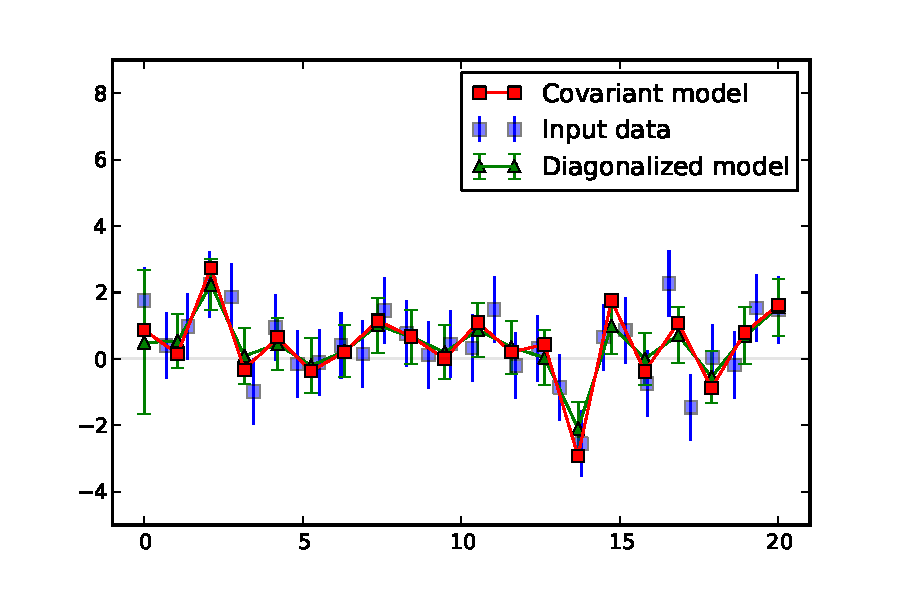
\includegraphics[width=0.8\textwidth]{plots/single_spec_1.pdf}
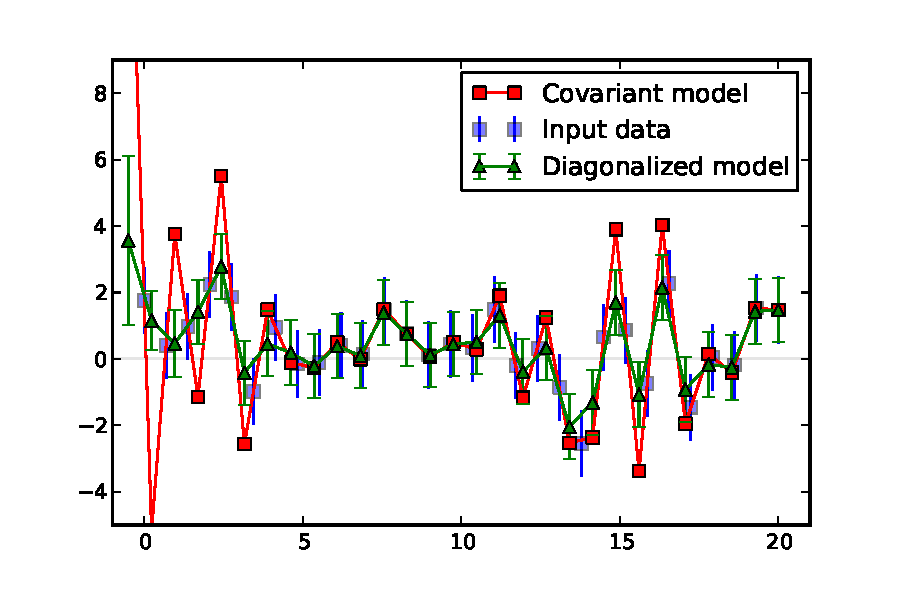
\includegraphics[width=0.8\textwidth]{plots/single_spec_2.pdf}
\caption{
Examples of resampling a spectrum (blue) to a different
wavelength grid (red) and then diagonalizing the covariance (green).
}
\label{fig:resample_spectrum}
\end{figure}

Figure~\ref{fig:resample_spectrum} shows examples of resampling an
input spectrum (blue squares) to a new wavelength grid (red squares)
for two different final wavelength grids.
The amount of covariance introduced is heavily dependent upon the
phasing of the input and output grids.  The green triangles show the
final spectrum resulting from diagonalizing the covariance.
Higher order interpolations such as cubic B-splines would have
less covariant ringing at the expense of spreading that covariance
over multiple bins.  The same procedure can be applied to diagonalize
any interpolation that can be parameterized as a matrix operation
$\f = \A \f^\prime$.

%-------------------------------------------------------------------------
\section{Coadding spectra}
\label{sec:coadd}

The same method can be used to coadd multiple spectra that are not natively
aligned on the same wavelength grid.
\begin{equation}
    \mathbf{g} = \mathbf{B} \f_\mathrm{coadd}
\end{equation}
where $\mathbf{g}$ is the concatenation of the individual input spectra,
and $\mathbf{B}$
is the combined transformation matrix from the new sampling to the original
individual samplings.  i.e. for $n$ spectra,
\begin{equation}
    \left[ \begin{array}{c}
        \f_1 \\
        \f_2 \\
        \vdots \\
        \f_n \\
    \end{array}
    \right] = \left[ \begin{array}{c}
        \A_1 \\
        \A_2 \\
        \vdots \\
        \A_n \\
    \end{array}
    \right] \f_\mathrm{coadd}
\end{equation}

The calculation proceeds as in the previous section, finding a resolution
matrix $\R$ that transforms the inverse covariance
$\Ci = \mathbf{B}^T \N^{-1} \mathbf{B}$ into a diagonal basis.

\subsection{Example: coadding spectra}

\begin{figure}[t]
\centering
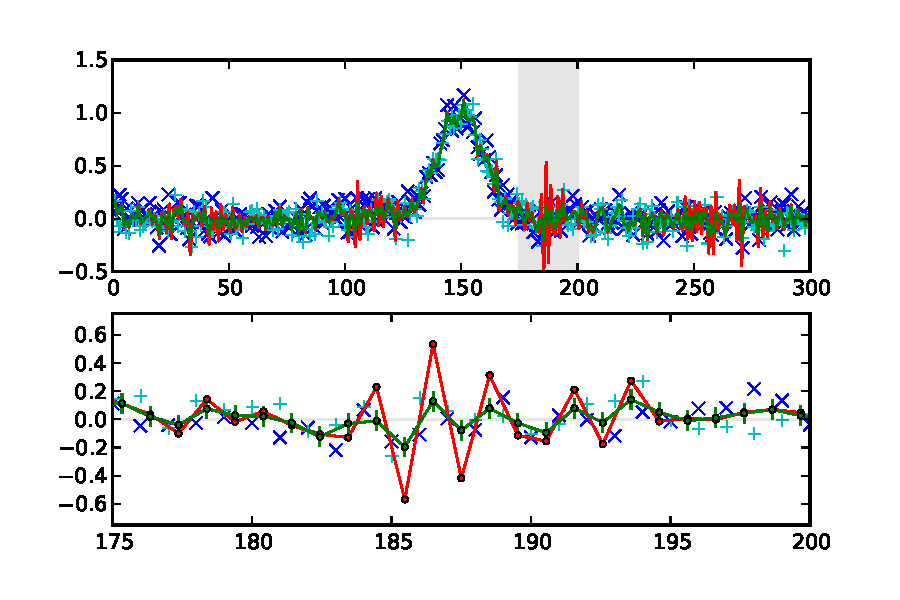
\includegraphics{plots/coadd_spectra.pdf}
\caption{
Example of coadding unaligned spectra onto a new wavelength grid.
Red shows the initial covariant resampling; green shows the diagonalized
coadded spectrum.  The bottom plot shows a zoom of the highlighted region
of the upper plot.
}
\label{fig:coadd_spectra}
\end{figure}

Figure~\ref{fig:coadd_spectra} shows an example of coadding unaligned spectra
onto a new wavelength grid.
Red shows the initial covariant resampling; green shows the diagonalized
coadded spectrum.  The original covariant coadd shows large oscillations
at certain wavelengths where the coadd overfits the data.  The diagonalized
coadded spectrum does not have this problem.

%-------------------------------------------------------------------------
\section{Resampling covariant spectra}

The same method can be used to simultaneously resample multiple
covariant spectra on to a common wavelength grid.

\begin{eqnarray}
    \left[ \begin{array}{c}
        \f_1 \\
        \f_2 \\
        \vdots \\
        \f_n \\
    \end{array}
    \right] & = & \left[ \begin{array}{c}
        \A_1 \\
        \A_2 \\
        \vdots \\
        \A_n \\
    \end{array}
    \right] \left[ \begin{array}{c}
        \f_1^\prime \\
        \f_2^\prime \\
        \vdots \\
        \f_n^\prime \\
    \end{array}    
    \right] \\
    \mathbf{g} & = & \mathbf{B} \mathbf{g}^\prime
\end{eqnarray}
In this case the $\f_i^\prime$ spectra are {\em different} spectra that
we wish to sample onto the same wavelength grid, {\it e.g.}, IFU spectra
of a galaxy for a data cube.  If the various spectra $\f_i$ are not noise
correlated with each other,
then the resampling of $\f^i = \A_i f_i^\prime$ proceeds identically to
section \ref{sec:single_spec}.  If they are noise correlated, then the
math is still the same but now $\N^{-1}$ is the full inverse noise covariance
of the multiple input spectra rather than a diagonal matrix.

\begin{figure}[t]
\centering
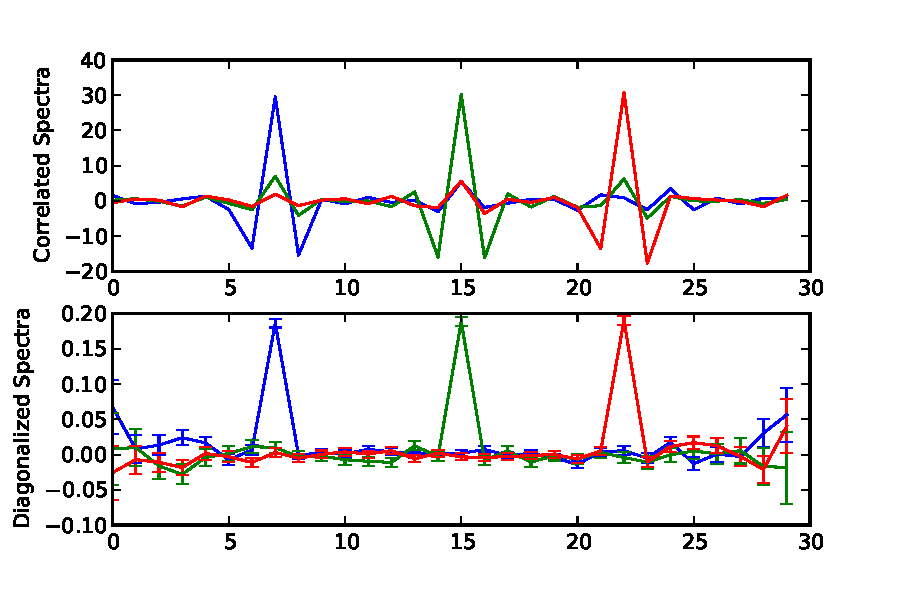
\includegraphics{plots/multiple_spectra.pdf}
\caption{
caption
}
\label{fig:multiple_spectra}
\end{figure}

Figure~\ref{fig:multiple_spectra} (top) shows 3 correlated spectra.
Within a spectrum, neighboring bins are negatively correlated, while
neighboring spectra are correlated with each other ---
blue is correlated with green; green is correlated with both blue and
red; and red is correlated with green.  The bottom plot of
figure~\ref{fig:multiple_spectra} shows the results of ...

%-------------------------------------------------------------------------
\appendix
\section{Solving for the resolution matrix $\R$}
\label{sec:solve_R}

This appendix shows how to solve for $\R$ given inverse covariance $\Ci$,
following Bolton \& Schlegel (2010) equations 10 through 16 with a few more 
steps filled in.

Start by finding the symmetric square root $\Q$ of $\Ci$ such that
$\Ci = \Q\Q$.  This can be found by eigen-decomposing $\Ci$ and
reconstructing with the square root of the eigenvalues:
\begin{eqnarray}
    \Ci & = & \mathbf{V} \mathbf{\Sigma} \mathbf{V}^T \\
    \Q & = & \mathbf{V} \mathbf{\Sigma}^{1/2} \mathbf{V}^T \\
    \Q\Q & = & \mathbf{V} \mathbf{\Sigma}^{1/2} \mathbf{V}^T
                \mathbf{V} \mathbf{\Sigma}^{1/2} \mathbf{V}^T \\
         & = & \mathbf{V} \mathbf{\Sigma} \mathbf{V}^T = \Ci
\end{eqnarray}
Next, define a normalization vector $\mathbf{s}$ using
\begin{equation}
    s_i = \sum_j Q_{ij} .
\end{equation}
The elements of the resolution matrix $\R$ are:
\begin{equation}
    R_{ij} = s_i^{-1} Q_{ij}~~~\mathrm{(no~sum)} .
\end{equation}
Thus by construction,
\begin{equation}
    \Ci = \R^T \tilde \Ci \R
\end{equation}
and
\begin{equation}
    \tilde \C = \R \C \R^T
\end{equation}
is a diagonal array with elements $s_i^{-2}$ giving the variance of the
transformed spectrum $\tilde \f = \R \f$.


\end{document}
